\documentclass{standalone}

\usepackage{tikz}
\usepackage{ctex}

\usetikzlibrary{shapes.misc}

\begin{document}
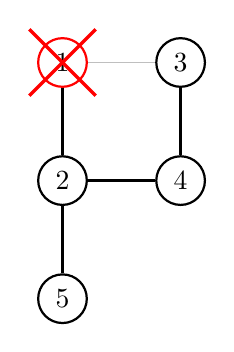
\begin{tikzpicture}[x=1.5cm,y=1.5cm]

\begin{scope}[every node/.style={draw},circle,thick]
    \node[draw=red] (A) at (0,2) {$1$};
    \node (B) at (0,1) {$2$};
    \node (C) at (1,2) {$3$};
    \node (D) at (1,1) {$4$};
    \node (E) at (0,0) {$5$};
\end{scope}

\draw[thick]
    (A) -- (B)
    (B) -- (D)
    (D) -- (C)
    (B) -- (E);

\draw[color=lightgray] (C) -- (A);

\node[cross out,draw=red,very thick,minimum size=8mm] at (A) {};

\end{tikzpicture}
\end{document}
